\documentclass[11pt]{article}
\usepackage[margin=1in]{geometry}
\usepackage{url}
\usepackage{amsmath}
\usepackage{amsfonts}
\usepackage{amssymb}
\usepackage{graphicx}
\usepackage{hyperref}
\usepackage{xcolor}
\usepackage{fontawesome5}
\usepackage{tikz}
\usepackage{pgfplots}
\usetikzlibrary{shapes,arrows,positioning,fit,backgrounds,calc}

\title{Machine Learning for Network Anomaly and Failure Detection}
\author{Michael Hernandez}
\date{September 27, 2025}

\begin{document}

% Cover Page
\begin{titlepage}
\centering
\vspace*{2cm}

{\Large \textbf{Machine Learning for Network Anomaly and Failure Detection}}

\vspace{1.5cm}

{\large CUNY School of Professional Studies}

\vspace{0.5cm}

{\large Michael Hernandez}

\vspace{0.5cm}

{\large IS 499 Information Systems Capstone}

\vspace{0.5cm}

{\large Professor John Bouma}

\vspace{0.5cm}

{\large September 27, 2025}

\vfill

\end{titlepage}

% Table of Contents
\tableofcontents
\newpage

\section{Introduction}

This paper examines machine learning techniques for detecting and localizing network anomalies and failures in large-scale environments, using data from BGP routing updates, SNMP metrics, and syslog messages.

Traditional network monitoring relies on threshold-based alerts from SNMP and syslog, often producing many false positives and offering little context for locating failures (Wang, 2020; Manna \& Alkasassbeh, 2019). Recent research has demonstrated that machine learning approaches applied to SNMP-MIB datasets can significantly improve anomaly detection accuracy and operational efficiency, with Random Forest classifiers achieving up to 100\% accuracy in identifying network failures (Manna \& Alkasassbeh, 2019). This project implements a dual-pipeline machine learning architecture with specialized algorithms for each data source: Matrix Profile for BGP time-series analysis (Scott et al., 2024) and Isolation Forest for SNMP hardware anomaly detection (Liu et al., 2008).

The system integrates two parallel detection pipelines for comprehensive network monitoring. The BGP pipeline uses Matrix Profile to detect routing anomalies in update streams, while the SNMP pipeline employs Isolation Forest to identify hardware and environmental failures in multi-dimensional feature spaces. Syslog messages provide temporal correlation signals, and multi-modal fusion reduces false positives by requiring confirmation across multiple data sources before generating alerts.

\section{Topic Description}

\subsection{In-depth Description of the Chosen Topic}

This project implements a dual-pipeline machine learning architecture for network anomaly detection and failure localization. The system employs specialized algorithms optimized for different data characteristics: Matrix Profile for BGP time-series analysis and Isolation Forest for SNMP high-dimensional feature analysis. This architecture enables comprehensive monitoring by processing BGP routing updates, SNMP hardware metrics, and syslog event messages through appropriate detection algorithms, then fusing signals for confirmed anomaly identification.

Border Gateway Protocol (BGP) is a standardized exterior gateway protocol that provides connectivity and fault tolerance for network devices on the Internet by exchanging routing and reachability information among autonomous systems. As a path-vector protocol, BGP maintains tables of IP network prefixes and makes routing decisions based on network policies configured by administrators. BGP is fundamental to Internet operation, dynamically updating routing information to adapt to network changes such as link failures or topology modifications. In the context of this project, BGP updates serve as critical indicators of network state changes, with anomalous BGP behavior often signaling underlying network issues (Scott et al., 2024).

The dual-pipeline architecture reflects the distinct characteristics of network telemetry data (Feltin et al., 2023). The BGP pipeline processes time-series data consisting of routing update sequences, where temporal patterns and sudden changes indicate network instability (Scott et al., 2024). The SNMP pipeline processes multi-dimensional feature vectors extracted from hardware metrics, where outliers in the feature space indicate component failures or environmental issues (Manna \& Alkasassbeh, 2019). This separation allows each pipeline to use algorithms optimized for its specific data type, while the fusion layer combines their outputs for comprehensive failure detection (Mohammed et al., 2021). Real-time processing requirements demand efficient algorithms: Matrix Profile operates with O(n log n) complexity for time-series analysis (Scott et al., 2024), while Isolation Forest provides O(n log n) outlier detection in high-dimensional spaces (Liu et al., 2008). Syslog messages provide temporal correlation signals that confirm anomalies detected in either pipeline.

The system uses Matrix Profile for time-series anomaly detection, Isolation Forest for unsupervised pattern recognition, and multi-modal fusion to combine signals from various sources. Matrix Profile is a data structure and algorithm that computes pairwise distances between all subsequences within a time series, enabling efficient identification of patterns (motifs) and anomalies (discords). By analyzing subsequences that deviate significantly from normal patterns, Matrix Profile provides unsupervised anomaly detection without requiring labeled training data (Scott et al., 2024). This approach is particularly effective for detecting subtle BGP routing anomalies that may indicate network failures or attacks. Isolation Forest complements Matrix Profile by providing anomaly detection in high-dimensional feature spaces through an ensemble of random decision trees that isolate anomalous data points. The algorithm operates on the principle that anomalies are easier to isolate than normal points, requiring fewer splits in the decision trees and thus having shorter path lengths from root to leaf (Liu et al., 2008). This makes Isolation Forest computationally efficient for detecting outliers in multi-dimensional feature vectors extracted from SNMP metrics without assuming specific data distributions. For syslog message analysis, deep learning approaches such as DeepSyslog demonstrate high effectiveness in detecting sequential anomalies through LSTM-based pattern recognition combined with sentence embeddings, achieving precision and recall rates exceeding 97\% on benchmark datasets (Zhou et al., 2022). Device role mapping provides topology awareness, categorizing network elements by function for context-aware anomaly localization.

\begin{figure}[h]
\centering
\resizebox{\textwidth}{!}{%
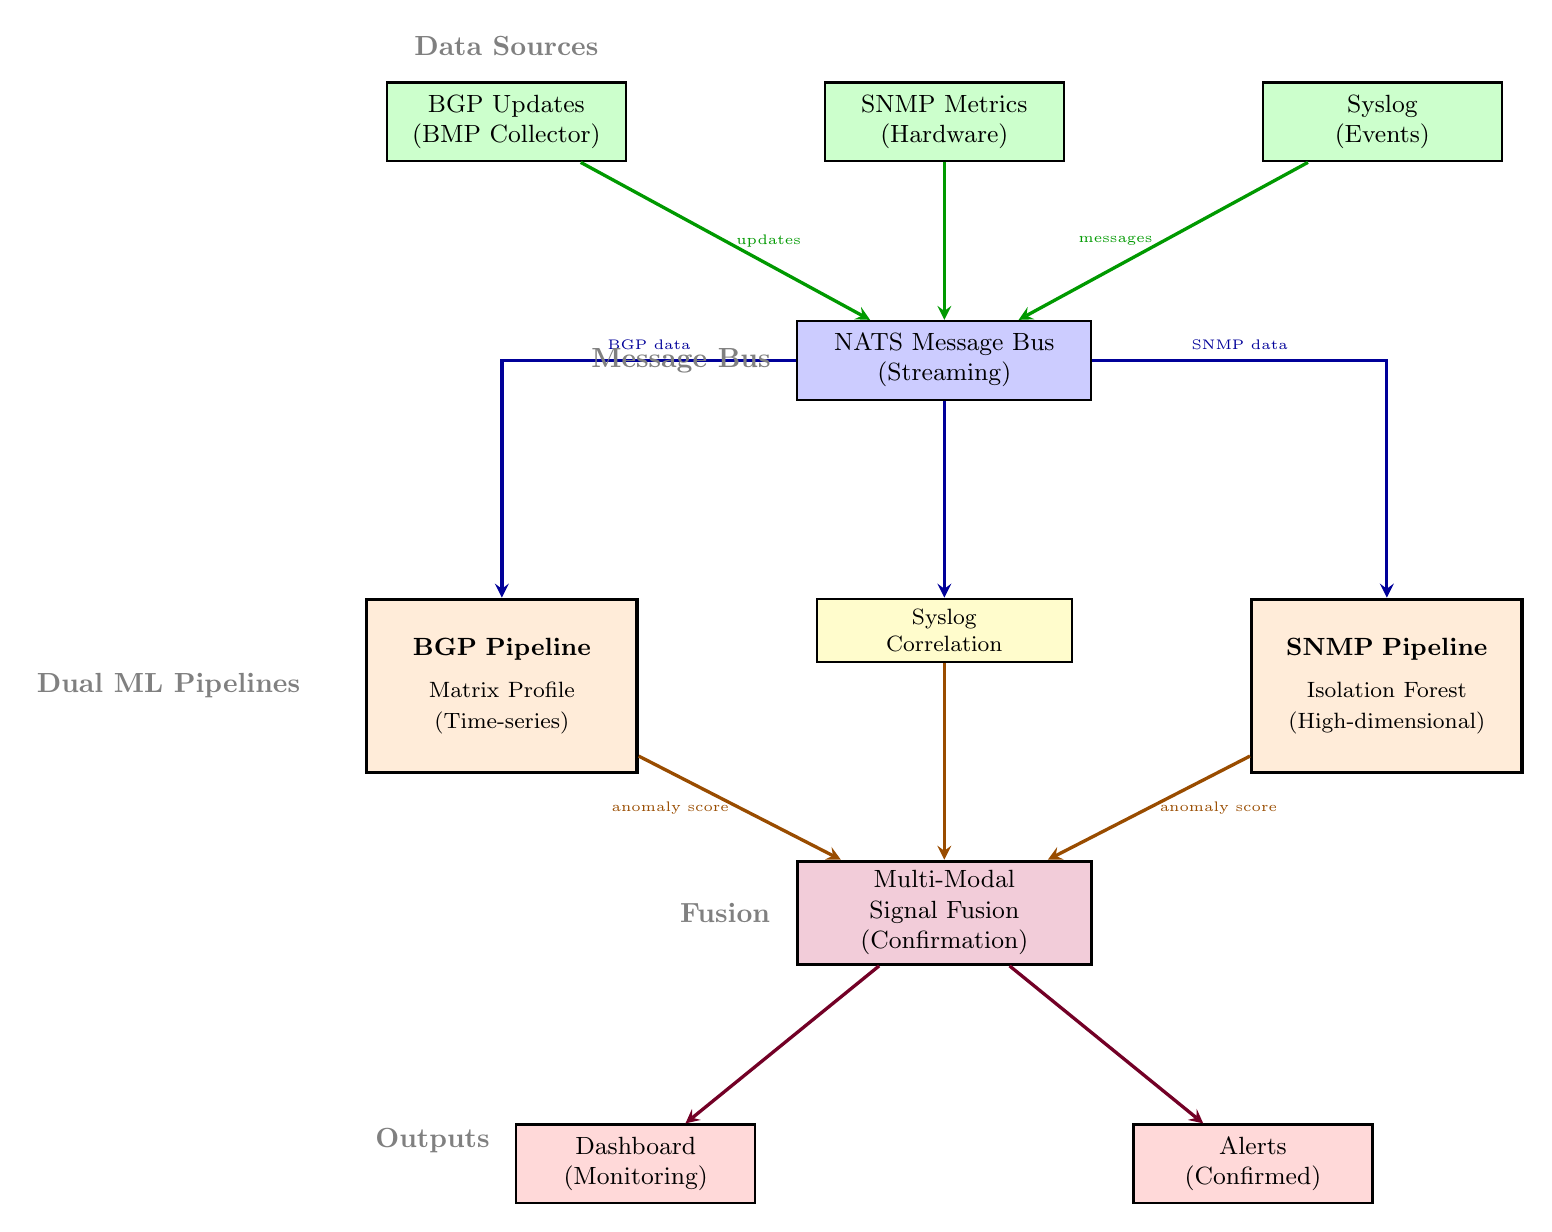
\begin{tikzpicture}[
    node distance=1.8cm and 2.5cm,
    source/.style={rectangle, draw=black, thick, fill=green!20, text width=2.8cm, align=center, minimum height=1cm, font=\small},
    bus/.style={rectangle, draw=black, thick, fill=blue!20, text width=3.5cm, align=center, minimum height=1cm, font=\small},
    pipeline/.style={rectangle, draw=black, very thick, fill=orange!15, text width=3.2cm, align=center, minimum height=2.2cm, font=\small},
    process/.style={rectangle, draw=black, thick, fill=yellow!20, text width=3cm, align=center, minimum height=0.8cm, font=\footnotesize},
    fusion/.style={rectangle, draw=black, very thick, fill=purple!20, text width=3.5cm, align=center, minimum height=1.2cm, font=\small},
    output/.style={rectangle, draw=black, thick, fill=red!15, text width=2.8cm, align=center, minimum height=1cm, font=\small},
    arrow/.style={->, >=stealth, line width=1.2pt},
]

% Layer 1: Data Sources
\node[source] (bgp) {BGP Updates\\(BMP Collector)};
\node[source, right=of bgp] (snmp) {SNMP Metrics\\(Hardware)};
\node[source, right=of snmp] (syslog) {Syslog\\(Events)};

% Layer 2: Message Bus
\node[bus, below=2cm of snmp] (nats) {NATS Message Bus\\(Streaming)};

% Layer 3: Dual Pipelines
\node[pipeline, below left=2.5cm and 2cm of nats] (bgp_pipe) {
    \textbf{BGP Pipeline}\\[0.2cm]
    \footnotesize Matrix Profile\\
    \footnotesize (Time-series)
};

\node[pipeline, below right=2.5cm and 2cm of nats] (snmp_pipe) {
    \textbf{SNMP Pipeline}\\[0.2cm]
    \footnotesize Isolation Forest\\
    \footnotesize (High-dimensional)
};

% Syslog correlation
\node[process, below=2.5cm of nats] (syslog_corr) {Syslog\\Correlation};

% Layer 4: Fusion
\node[fusion, below=2.5cm of syslog_corr] (fusion) {Multi-Modal\\Signal Fusion\\(Confirmation)};

% Layer 5: Outputs
\node[output, below left=2cm and 0.5cm of fusion] (dashboard) {Dashboard\\(Monitoring)};
\node[output, below right=2cm and 0.5cm of fusion] (alerts) {Alerts\\(Confirmed)};

% Arrows - Sources to Bus
\draw[arrow, green!60!black] (bgp) -- node[right, font=\tiny] {updates} (nats);
\draw[arrow, green!60!black] (snmp) -- (nats);
\draw[arrow, green!60!black] (syslog) -- node[left, font=\tiny] {messages} (nats);

% Arrows - Bus to Pipelines
\draw[arrow, blue!60!black] (nats) -| node[near start, above, font=\tiny] {BGP data} (bgp_pipe);
\draw[arrow, blue!60!black] (nats) -| node[near start, above, font=\tiny] {SNMP data} (snmp_pipe);
\draw[arrow, blue!60!black] (nats) -- (syslog_corr);

% Arrows - Pipelines to Fusion
\draw[arrow, orange!60!black] (bgp_pipe) -- node[left, font=\tiny] {anomaly score} (fusion);
\draw[arrow, orange!60!black] (snmp_pipe) -- node[right, font=\tiny] {anomaly score} (fusion);
\draw[arrow, orange!60!black] (syslog_corr) -- (fusion);

% Arrows - Fusion to Outputs
\draw[arrow, purple!60!black] (fusion) -- (dashboard);
\draw[arrow, purple!60!black] (fusion) -- (alerts);

% Labels
\node[above=0.2cm of bgp, font=\normalsize\bfseries, text=gray] {Data Sources};
\node[left=0.2cm of nats, font=\normalsize\bfseries, text=gray] {Message Bus};
\node[left=0.2cm of bgp_pipe, font=\normalsize\bfseries, text=gray, xshift=-0.5cm, align=center] {Dual ML Pipelines};
\node[left=0.2cm of fusion, font=\normalsize\bfseries, text=gray] {Fusion};
\node[left=0.2cm of dashboard, font=\normalsize\bfseries, text=gray, yshift=0.3cm] {Outputs};

\end{tikzpicture}
}
\caption{Dual-Pipeline Architecture: BGP updates processed by Matrix Profile (time-series), SNMP metrics by Isolation Forest (high-dimensional), with syslog correlation. Multi-modal fusion confirms anomalies across sources before alerting.}
\label{fig:architecture}
\end{figure}

Figure \ref{fig:architecture} illustrates the dual-pipeline ML architecture showing how BGP and SNMP data flow through specialized detection algorithms before multi-modal fusion.

\subsection{Why This Topic Was Chosen}

This topic was chosen due to fundamental challenges in network operations where traditional monitoring systems often produce many false positives yet miss critical anomalies (Skazin, 2021). Modern network architectures, such as large-scale BGP-routed environments with anycast services and overlay networks, surpass the capabilities of threshold-based alerting systems, requiring more sophisticated approaches to anomaly detection and failure localization.

Network operations centers managing enterprise-scale infrastructures face several critical challenges. Alert fatigue from excessive false positives leads to decreased operator responsiveness, while the lack of contextual information makes it difficult to distinguish routine network variations from genuine anomalies requiring immediate attention. Manual correlation of events across thousands of devices becomes impractical, resulting in extended mean time to resolution (MTTR) for incidents. Machine learning approaches offer the potential to address these challenges through automated pattern recognition and anomaly detection (Mohammed et al., 2021).

Consider a representative use case: a large enterprise network with multiple data centers connected via BGP-routed fabric experiences an intermittent link failure that causes route flapping. Traditional monitoring generates hundreds of alerts from affected routers, but provides no indication of the failure's root cause or scope. Network engineers must manually correlate BGP update logs, SNMP interface counters, and syslog messages across dozens of devices to identify the failing link and assess impact on services. This manual investigation process can take extended periods during critical outages, contributing to increased mean time to resolution (MTTR). An ML-based system using Matrix Profile analysis can automatically detect the anomalous pattern in BGP update frequency, correlate it with SNMP interface error counters, and use topology awareness to localize the failure to the specific failing link, significantly reducing investigation time and improving operational efficiency (Mohammed et al., 2021).

The selection of Matrix Profile and Isolation Forest as core algorithms reflects specific technical requirements. Matrix Profile provides efficient subsequence similarity analysis for time-series data without requiring labeled training examples, making it suitable for detecting novel anomaly patterns in BGP update streams. The algorithm computes a distance profile that identifies subsequences with unusual characteristics relative to the rest of the time series, with computational complexity of O(n log n) enabling real-time processing. Isolation Forest complements this approach by providing unsupervised anomaly detection in high-dimensional feature spaces extracted from SNMP metrics. By constructing random decision trees that isolate anomalous points with fewer splits than normal points, Isolation Forest efficiently identifies outliers in multi-modal feature vectors without assuming specific distribution patterns. For syslog analysis, while deep learning methods such as DeepSyslog have demonstrated superior performance on log anomaly detection benchmarks with precision and recall both exceeding 97\% through LSTM-based sequential pattern recognition (Zhou et al., 2022), the current implementation utilizes pattern-based correlation to maintain system simplicity and real-time processing requirements. This approach allows the syslog component to provide temporal correlation signals for multi-modal fusion while keeping computational overhead minimal. Together, these techniques enable robust unsupervised anomaly detection across diverse data sources, with the architecture designed to accommodate future integration of LSTM-based syslog analysis for enhanced sequential pattern detection.

\section{Problem Description}

\subsection{Detailed Content Around the Problems Being Solved}

The problem I am trying to solve is the inadequacy of traditional network monitoring systems in detecting and localizing network anomalies and failures in large-scale, complex environments. This project addresses alert fatigue from false positives, delayed failure detection, and insufficient context for assessing failure scope and impact. Traditional SNMP threshold alerts and syslog pattern matching produce excessive benign alerts and miss subtle anomalies, while conventional log analysis lacks the sophistication needed for modern networks (Allagi \& Rachh, 2019). Research has shown that among SNMP-MIB groups, the Interface and IP groups are most affected by various failure types and anomalies, while ICMP, TCP, and UDP groups are less impacted (Manna \& Alkasassbeh, 2019), highlighting the need for targeted monitoring strategies that can quickly identify scope and severity.

These problems arise from the complexity of modern network architectures and the limits of traditional monitoring. Large networks have thousands of devices with various failure modes, such as hardware issues, environmental factors, and routing anomalies. Current systems lack topology awareness and multi-modal data correlation, making it hard to separate normal variations from true anomalies.

These issues vary by network environment but are common in large-scale BGP-routed networks with anycast services and overlay technologies. Enterprise networks requiring dedicated network operations centers (NOCs) with multiple engineers often span thousands of devices across campus and data center environments, making manual correlation across devices and services impractical (Skazin, 2021).

Solving these problems is urgent as they affect network reliability and efficiency. Detection delays extend resolution times, alert fatigue risks missed critical issues, and lacking automated correlation means failures are often found only after escalating to service-impacting levels.

\subsection{Current Network Monitoring Limitations}

Current network monitoring systems exhibit fundamental limitations in their design and operational effectiveness. Traditional approaches based on SNMP threshold monitoring and syslog pattern matching can detect hard failures such as interface down events or device unreachability, but they produce excessive alerts for benign events while simultaneously missing subtle anomalies that may indicate developing problems. Research has shown that conventional log analysis methods lack the sophistication needed for modern network environments, with traditional rule-based systems struggling to adapt to the dynamic nature of large-scale networks (Allagi \& Rachh, 2019). As a result, operations teams experience alert fatigue from false positives while critical anomalies go undetected until they escalate to service-impacting failures (Mohammed et al., 2021).

The insufficiency of current monitoring systems manifests in several specific ways. First, threshold-based alerting requires manual configuration of acceptable ranges for each monitored metric, but optimal thresholds vary based on device role, time of day, and network load patterns. Static thresholds either trigger excessive false positives during normal traffic variations or fail to detect anomalies that remain below configured thresholds. Second, current systems lack correlation capabilities across different data sources. A gradual increase in BGP update frequency combined with rising SNMP interface error counters and specific syslog error patterns may collectively indicate an impending link failure, but traditional monitoring evaluates each metric independently without cross-modal correlation. Third, existing systems provide no topology awareness or understanding of failure propagation patterns. When a core aggregation switch experiences issues, downstream devices also generate alerts, but traditional monitoring cannot distinguish the root cause from cascading effects (Skazin, 2021).

The scale and complexity of modern networks intensify these monitoring challenges. Large BGP-routed environments often include thousands of devices, anycast services, and global VXLAN overlays, introducing multiple failure modes that demand varied detection and response strategies. Studies of SNMP-MIB data have revealed that among all monitored groups, the Interface and IP groups are most affected by various failure types and anomalies, while ICMP, TCP, and UDP groups show less sensitivity to network issues (Manna \& Alkasassbeh, 2019). This differential sensitivity requires intelligent monitoring that can focus on relevant metrics rather than treating all data sources equally.

Research demonstrates that machine learning approaches can significantly improve upon traditional methods. Classifiers such as Random Forest and Decision Trees applied to SNMP-MIB datasets have achieved high accuracy in identifying network failures, suggesting that supervised and unsupervised learning can extract patterns from network telemetry that static thresholds cannot capture (Manna \& Alkasassbeh, 2019). Furthermore, the integration of multiple data modalities through feature selection and correlation enables more comprehensive anomaly detection than any single data source alone (Feltin et al., 2023). These findings motivate the development of ML-based monitoring systems that can adapt to network dynamics, correlate multi-modal signals, and provide topology-aware failure localization.

\section{Analysis}

\subsection{Testing Infrastructure and Evaluation Framework}

The system is validated using realistic simulated data that provides controlled BGP and SNMP scenarios for testing the dual-pipeline anomaly detection architecture.

\begin{figure}[h]
\centering
\resizebox{0.9\textwidth}{!}{%
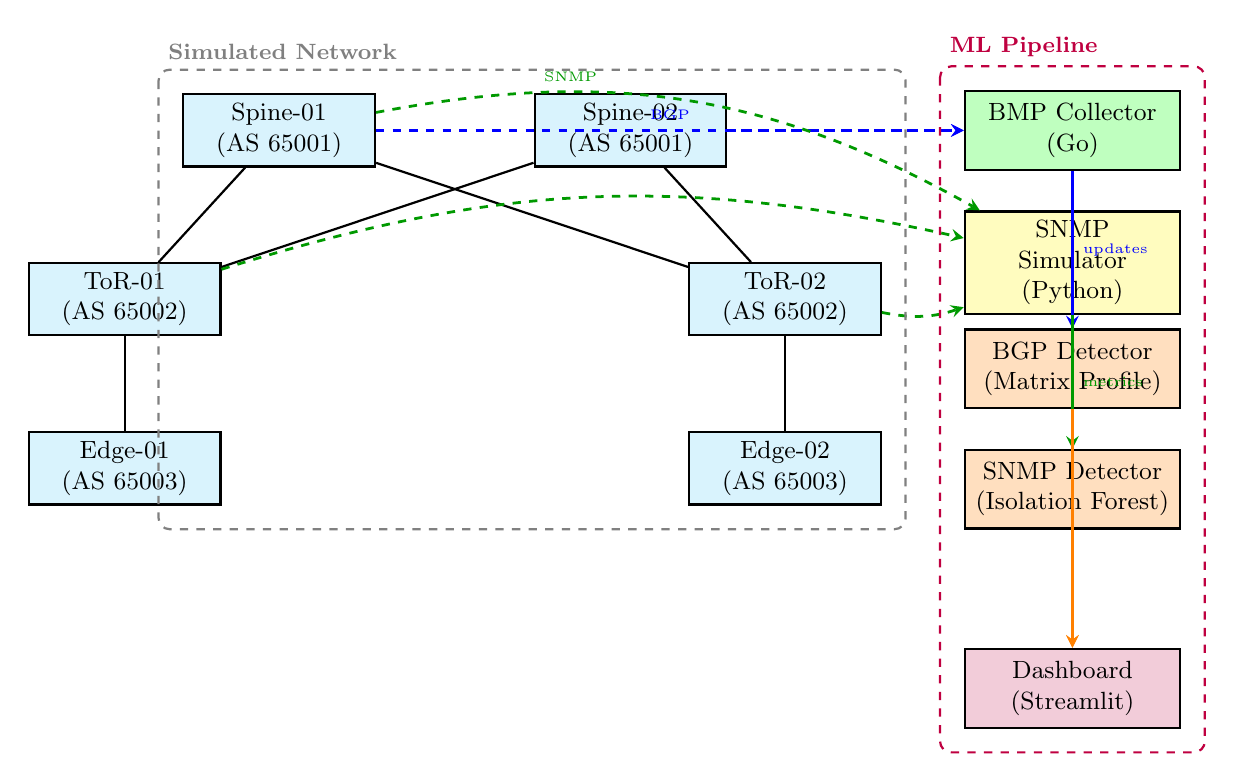
\begin{tikzpicture}[
    node distance=1.5cm and 2cm,
    device/.style={rectangle, draw=black, thick, fill=cyan!15, text width=2.2cm, align=center, minimum height=0.9cm, font=\small},
    collector/.style={rectangle, draw=black, thick, fill=green!25, text width=2.5cm, align=center, minimum height=1cm, font=\small},
    detector/.style={rectangle, draw=black, thick, fill=orange!25, text width=2.5cm, align=center, minimum height=1cm, font=\small},
    simulator/.style={rectangle, draw=black, thick, fill=yellow!25, text width=2.5cm, align=center, minimum height=1cm, font=\small},
    arrow/.style={->, >=stealth, line width=1pt},
]

% Network Devices (Simulated)
\node[device] (spine1) {Spine-01\\(AS 65001)};
\node[device, right=of spine1] (spine2) {Spine-02\\(AS 65001)};
\node[device, below left=1.2cm and -0.5cm of spine1] (tor1) {ToR-01\\(AS 65002)};
\node[device, below right=1.2cm and -0.5cm of spine2] (tor2) {ToR-02\\(AS 65002)};
\node[device, below=1.2cm of tor1] (edge1) {Edge-01\\(AS 65003)};
\node[device, below=1.2cm of tor2] (edge2) {Edge-02\\(AS 65003)};

% Network connections
\draw[line width=0.8pt] (spine1) -- (tor1);
\draw[line width=0.8pt] (spine1) -- (tor2);
\draw[line width=0.8pt] (spine2) -- (tor1);
\draw[line width=0.8pt] (spine2) -- (tor2);
\draw[line width=0.8pt] (tor1) -- (edge1);
\draw[line width=0.8pt] (tor2) -- (edge2);

% Data Collectors
\node[collector, right=3cm of spine2] (bmp) {BMP Collector\\(Go)};
\node[simulator, below=0.5cm of bmp] (snmp_sim) {SNMP\\Simulator\\(Python)};

% Detection Pipelines
\node[detector, below=2cm of bmp] (bgp_detect) {BGP Detector\\(Matrix Profile)};
\node[detector, below=0.5cm of bgp_detect] (snmp_detect) {SNMP Detector\\(Isolation Forest)};

% Dashboard
\node[detector, fill=purple!20, below=1.5cm of snmp_detect] (dashboard) {Dashboard\\(Streamlit)};

% Arrows - Devices to Collectors
\draw[arrow, blue, dashed] (spine1) -- node[above, font=\tiny] {BGP} (bmp);
\draw[arrow, blue, dashed] (spine2) -- (bmp);
\draw[arrow, green!60!black, dashed] (spine1) to[bend left=20] node[above, font=\tiny, pos=0.3] {SNMP} (snmp_sim);
\draw[arrow, green!60!black, dashed] (tor1) to[bend left=15] (snmp_sim);
\draw[arrow, green!60!black, dashed] (tor2) to[bend right=15] (snmp_sim);

% Arrows - Collectors to Detectors
\draw[arrow, blue] (bmp) -- node[right, font=\tiny] {updates} (bgp_detect);
\draw[arrow, green!60!black] (snmp_sim) -- node[right, font=\tiny] {metrics} (snmp_detect);

% Arrows - Detectors to Dashboard
\draw[arrow, orange] (bgp_detect) -- (dashboard);
\draw[arrow, orange] (snmp_detect) -- (dashboard);

% Test network boundary
\draw[dashed, gray, thick, rounded corners] ($(spine1.north west)+(-0.3,0.3)$) rectangle ($(edge2.south east)+(0.3,-0.3)$);
\node[above right, font=\footnotesize\bfseries, text=gray] at ($(spine1.north west)+(-0.3,0.3)$) {Simulated Network};

% Test harness boundary
\draw[dashed, purple, thick, rounded corners] ($(bmp.north west)+(-0.3,0.3)$) rectangle ($(dashboard.south east)+(0.3,-0.3)$);
\node[above right, font=\footnotesize\bfseries, text=purple] at ($(bmp.north west)+(-0.3,0.3)$) {ML Pipeline};

\end{tikzpicture}
}
\caption{Test Environment: Simulated network with 6 devices (2 spine, 2 ToR, 2 edge) generating realistic BGP updates and SNMP metrics. Data simulators produce BMP-format routing updates and hardware telemetry that feed the dual-pipeline ML system for validation testing.}
\label{fig:lab}
\end{figure}

Figure \ref{fig:lab} shows the test environment used for validation, consisting of realistic data simulators generating BGP updates and SNMP metrics, integrated with the dual-pipeline ML detection system.

\textcolor{red}{\textbf{[SECTION PLACEHOLDER - Additional analysis content to be completed]}}

This section will include analysis of how the topic was chosen, how problems were identified, how solutions fulfill operational and strategic goals, implementation timeline, and current implementation status.

\section{Research}

\textcolor{red}{\textbf{[SECTION PLACEHOLDER - TO BE COMPLETED]}}

This section will include coursework background and supporting references that provide the research foundation for the project.

\section{References}

\begin{thebibliography}{9}

\bibitem{cheng2021}
Cheng, M., Li, Q., Lv, J., Liu, W., \& Wang, J. (2021).
Multi-Scale LSTM Model for BGP Anomaly Classification.
\textit{IEEE Transactions on Services Computing}, 14(3), 765--778.
Available at: \href{https://doi.org/10.1109/TSC.2018.2824809}{https://doi.org/10.1109/TSC.2018.2824809}

\bibitem{mohammed2021}
Mohammed, S. A., Mohammed, A. R., Côté, D., \& Shirmohammadi, S. (2021).
A machine-learning-based action recommender for Network Operation Centers.
\textit{IEEE Transactions on Network and Service Management}, 18(3), 2702--2713.
Available at: \href{https://doi.org/10.1109/TNSM.2021.3095463}{https://doi.org/10.1109/TNSM.2021.3095463}

\bibitem{scott2024}
Scott, B., Johnstone, M. N., Szewczyk, P., \& Richardson, S. (2024).
Matrix Profile data mining for BGP anomaly detection.
\textit{Computer Networks}, 242, 110257.

\bibitem{tan2024}
Tan, Y., Huang, W., You, Y., Su, S., \& Lu, H. (2024).
Recognizing BGP Communities Based on Graph Neural Network.
\textit{IEEE Network}, 38(6), 232--238.
Available at: \href{https://doi.org/10.1109/MNET.2024.3414113}{https://doi.org/10.1109/MNET.2024.3414113}

\bibitem{allagi2019}
Allagi, S., \& Rachh, R. (2019).
Analysis of Network log data using Machine Learning.
\textit{2019 IEEE 5th International Conference for Convergence in Technology (I2CT)}, 1--3.
Available at: \href{https://doi.org/10.1109/I2CT45611.2019.9033528}{https://doi.org/10.1109/I2CT45611.2019.9033528}

\bibitem{skazin2021}
Skazin, A. (2021).
Detection of network anomalies in log files.
\textit{IOP Conference Series: Materials Science and Engineering}, 1069(1), 012021.
Available at: \href{https://doi.org/10.1088/1757-899X/1069/1/012021}{https://doi.org/10.1088/1757-899X/1069/1/012021}

\bibitem{feltin2023}
Feltin, T., Cordero Fuertes, J. A., Brockners, F., \& Clausen, T. H. (2023).
Understanding Semantics in Feature Selection for Fault Diagnosis in Network Telemetry Data.
\textit{NOMS 2023-2023 IEEE/IFIP Network Operations and Management Symposium}, 1--9.
Available at: \href{https://doi.org/10.1109/NOMS56928.2023.10154455}{https://doi.org/10.1109/NOMS56928.2023.10154455}

\bibitem{wang2020}
Wang, H. (2020).
Improvement and implementation of Wireless Network Topology System based on SNMP protocol for router equipment.
\textit{Computer Communications}, 151, 10--18.
Available at: \href{https://doi.org/10.1016/j.comcom.2020.01.001}{https://doi.org/10.1016/j.comcom.2020.01.001}

\bibitem{manna2019}
Manna, A., \& Alkasassbeh, M. (2019).
Detecting network anomalies using machine learning and SNMP-MIB dataset with IP group.
\textit{arXiv preprint arXiv:1906.00863}.
Available at: \href{https://arxiv.org/abs/1906.00863}{https://arxiv.org/abs/1906.00863}

\bibitem{liu2008}
Liu, F. T., Ting, K. M., \& Zhou, Z.-H. (2008).
Isolation Forest.
\textit{2008 Eighth IEEE International Conference on Data Mining}, 413--422.
Available at: \href{https://doi.org/10.1109/ICDM.2008.17}{https://doi.org/10.1109/ICDM.2008.17}

\bibitem{zhou2022}
Zhou, J., Qian, Y., Zou, Q., Liu, P., \& Xiang, J. (2022).
DeepSyslog: Deep Anomaly Detection on Syslog Using Sentence Embedding and Metadata.
\textit{IEEE Transactions on Information Forensics and Security}, 17, 3051--3066.
Available at: \href{https://doi.org/10.1109/TIFS.2022.3198188}{https://doi.org/10.1109/TIFS.2022.3198188}

\end{thebibliography}

\end{document}
